% !TeX spellcheck = cs_CZ
% Musilova2009MA1

\begin{example}\label{mai:exam001}
  \textbf{Parametrické vyjádření přímky}\newline
  \emph{Přímka} — jednorozměrný lineární útvar v jednorozměrném prostoru \(\mathcal{R}^1\), 
  dvojrozměrném prostoru \(\mathcal{R}^2\), trojrozměrném prostoru \(\mathcal{R}^3\) (nebo i 
  n-rozměrném prostoru \(\mathcal{R}^n\)), je určena dvěma body, třeba \(A\) a \(B\), nebo
  ekvivalentně, bodem \(A\) a \emph{směrovým} vektorem \(\vec{u}\) (obr. \ref{mai:fig000}). 
  Je-li \(X\) obecným bodem na této přímce, je vektor \(\overrightarrow{AX}\) rovnoběžný, tj. 
  \emph{kolineární}, se směrovým vektorem \(\vec{u}\). (Jako směrový můžeme samozřejmě 
  použít i vektor \(\overrightarrow{AB}\).) Vektor \(\overrightarrow{AX}\) má tedy s vektorem 
  \(\vec{u}\) stejný směr, lišit se může velikostí nebo orientací. Tuto skutečnost zapíšeme 
  tak, že \(\overrightarrow{AX}\) je \emph{t}-násobkem vektorů \(\vec{u}\),
  \begin{equation*}
  \overrightarrow{AX} = t \cdot \vec{u}.
  \end{equation*}
  {\centering
    \captionsetup{type=figure}
    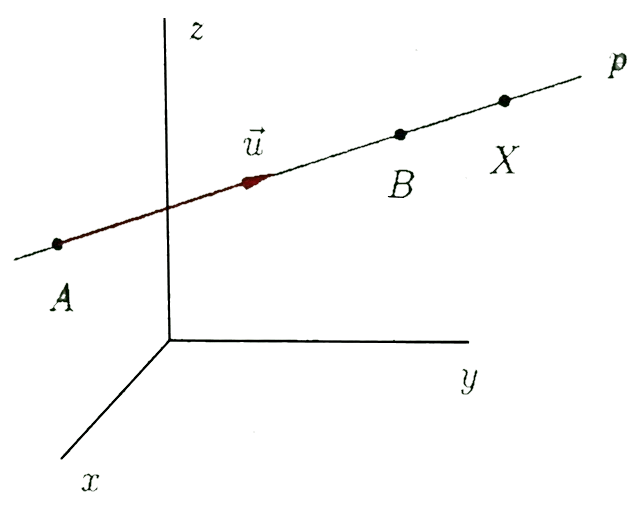
\includegraphics[width=0.5\linewidth]{mai_fig000.png}
    \captionof{figure}{Zadáni přímky. \cite[s.~1]{Musilova2009MA1}
    \label{mai:fig000}}
    \par}        
  Veličinou \(t\), takzvaným \emph{parametrem}, který může nabývat všech reálných hodnot, 
  \(t\in\mathcal{R}\), dokážeme popsat všechny vektory \(\overrightarrow{AX}\), jejichž 
  koncový bod \(X\) leží na přímce \(p\). Naopak, žádné jiné body \(X\) než ty, které leží na 
  přímce \(p\), tuto vlastnost nemají. S označením bodů \(A\), \(X\), resp. vektorů 
  \(\vec{u}\), \(\overrightarrow{AX}\) kartézskými souřadnicemi, resp. složkami
  \begin{align*}
                    A &= (x_A,y_A, z_A), \\ 
                    X &=(x,y,z),         \\
              \vec{u} &= (u_1,u_2,u_3),  \\ 
  \overrightarrow{AX} &= (x - x_A, y - y_1A, z-z_A),
  \end{align*}
  dostáváme \textbf{parametrické vyjádřeni přímky} \(p\) ve tvaru
  \begin{equation}
    p = \left\{(x,y,z)\in\mathcal{R}^3\,|\,
    \begin{matrix}
      x = x_A + tu_1,        \\
      y = y_A + tu_2,        \\
     z = z_A + tu_3,
    \end{matrix}
    \;t\in\mathcal{R}
    \right\}. \label{MAI:eq_M001}
  \end{equation}
\end{example}
\normalsize